\section{Large-scale data processing with MapReduce}
When we have a lot of data, we must exploit multiple machines, so larger architectures that support parallelization, both on the computation and on the read/write operations. In this sense, some standard architectures are \textbf{commodity clusters}, which are standard servers that scale the computation up on different machines, and \textbf{Gigabit Ethernet interconnections.}

\subsection{Commodity clusters}

\begin{figure}[h!]
		\centering
		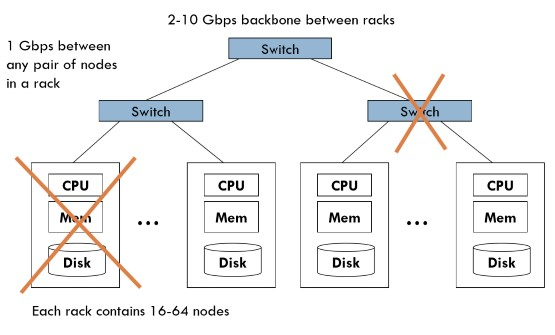
\includegraphics[scale = 2.0]{img/cluster.jpg}
        \label{cl arch}
        \caption{Cluster architecture}
\end{figure}

As we can see, two main failures may happen:

\begin{itemize}
    \item A failure in the \textbf{network}, after which some nodes are not reachable anymore;
    \item A failure on a \textbf{machine}.
\end{itemize}

In general, handling failures is difficult, since they're extremely frequent, so an important property of the cluster is to be \textbf{failure resilient}. In particular, if we address the problem of a \textit{machine failure}, we have a solution represented by the \textbf{Distributed File System}, which provides a global file namespace and it supports huge files (100 of GBs to TBs): in this case, data is rarely updated in place, and \textbf{reads} and \textbf{appends} are common. Some examples of such DFS are \textit{Google GFS} and \textit{Hadoop HDFS}

In particular, the Hadoop DFS is composed of the following entities:

\begin{itemize}
    \item \textbf{Chunk servers}, which contain the splitted file and serve the \textit{master node}. Each chunk is typically 16-64MB, and it is replicated 2x or 3x, so the \textbf{replication} is at \textbf{chunk level}. Note that the HDFS tries to keep the replicas in different racks;
    \item \textbf{Master node} (or \textbf{Name node}), which stores all the metadata and takes care of giving the user a unique FS, and it keeps track of all the chunk servers. The mater node might be replicated;
    \item Client library for file access, which talks to the master node to find the chunk servers and connects directly to chunk servers to access data.
\end{itemize}

The operations that are supported by the HDFS are \textbf{concurrent reads} and \textbf{single write} operations, which are implemented as append operations.

Two very important files in the HDFS are:

\begin{itemize}
    \item The \textbf{sequence file}, which is persistent data structure for binary key-value pairs. This file can be written only by using the \textit{append()} method, and can be read only by using the \textit{next()} method;
    \item The \textbf{map file}, which represents a higher-level file and it is a \textbf{sorted sequence file} with an \textbf{index} to support lookups by key. Thus, in this case the file can be read by using \textit{next()} or \textit{get()} (by key). Notice that the lookup by key is implemented with two sequence files: \textit{Index} and \textit{Data}, where the \textit{Index} file must be loaded in memory for random lookups.

    \begin{figure}[h!]
		\centering
		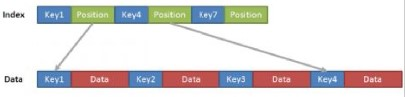
\includegraphics[scale = 2.0]{img/index map file.jpg}
        \label{sequence map files}
        \caption{\textit{Index} and \textit{Data} files}
    \end{figure}
\end{itemize}

Finally, notice that the \textbf{replication of data three times} is a robust guard against loss of data due to uncorrelated node failures: for a large cluster, the probability of losing a block during one year is less than 0.005. The key understanding is that about 0.8 percent of nodes fail each month, so for the sample of large clusters, a node or two is lost everyday.

\subsection{MapReduce}
\textbf{MapReduce} represents a "novel" programming paradigm, which is based on top of \textit{<key,value>} pairs, where the \textit{keys} and the \textit{values} are \textbf{user-defined}, so they can have any type. This framework is essentially based on two functions:

\begin{itemize}
    \item \textbf{Map}, which takes as input a key-value pair $(k_1, v_1)$, and produces as output an intermediate data $v_2$ labeled with a key $k_2$:

    $$
    \text{Map}(k_1, v_1) = \text{list}(k_2, v_2)
    $$
    
    \item \textbf{Reduce}, which given every data $\text{list}(v_2)$ associated with a key $k_2$ (so we suppose that we can execute multiple \textit{Map} operations on the same data), it produces the output of the algorithm $\text{list}(k_3, v_3)$, so its functioning is pretty similar to a GroupBy.

    $$
    \text{Reduce}(k_2, \text{list}(v_2)) = \text{list}(k_3, v_3)
    $$
\end{itemize}

If we put all in parallel, we have a set of \textbf{mappers} and a set of \textbf{reducers}:

\begin{enumerate}
    \item A \textbf{mapper} processes only a split of the input, which may be distributed across several machines;

    $$
    \text{Map}(k_1, v_1) = \text{list}(k_2, v_2)
    $$
    
    \item A \textbf{shuffle} phase transfers the data associated with a given key from the \textit{mappers} to the proper \textit{reducer}, so that the reducer will receive data sorted by key;
    \item A \textbf{reducer} produces only a portion of the output associated with a given set of keys. Notice that \textit{reducers} can run in parallel.

    $$
    \text{Reduce}(k_2, \text{list}(v_2)) = \text{list}(k_3, v_3)
    $$
    
\end{enumerate}

\underline{Example: WordCount using MapReduce}

Picture \ref{wc code} show the code of the Map and Reduce functions for the word count problem.

\begin{figure}[h!]
		\centering
		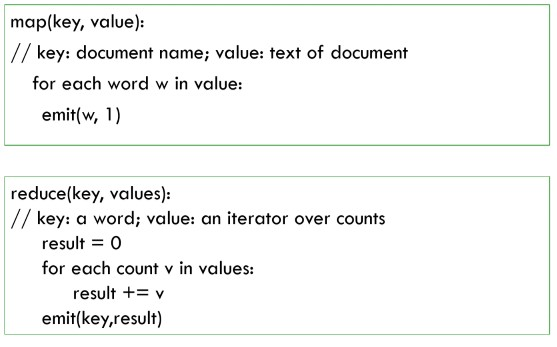
\includegraphics[scale = 2.0]{img/word count code.jpg}
        \label{wc code}
        \caption{Map and Reduce functions for word count problem}
\end{figure}

As we can see, the Map function produces a (word,1) pair for each of the word in the document, while the Reduce function receives in input a word and a list of 1's, and produce in output a (word,count) pair.

Picture \ref{wc scheme} shows the execution of the MapReduce framework for word counting.

\begin{figure}[h!]
		\centering
		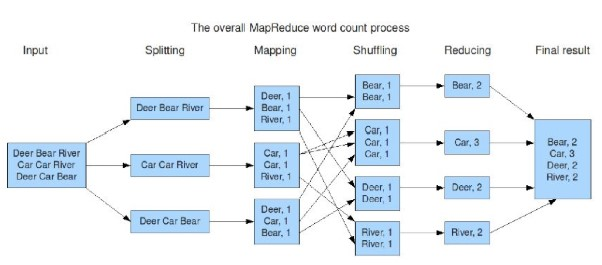
\includegraphics[scale = 2.0]{img/word count scheme.jpg}
        \label{wc scheme}
        \caption{Execution scheme of MapReduce for word counting}
\end{figure}

As we can see, the text is splitted into 3 chunks: the Map function of each chunk produces a (word,1) pair for each word of the input. Then, the Shuffle phase implements a GroupBy over the output of the Map functions, and produces a pair composed by a word and a list of 1's, which represents the input of the Reduce function. Finally, the output provides the count for each word of the input. Notice that the only operations that the user has to implement are the one from the Split phase to the Map phase, and from the Shuffle phase to the Reduce phase, since all the others belong to the MapReduce framework.

\subsubsection{Architecture}

Picture \ref{mr arch} shows the general architecture of the MapReduce framework.

\begin{figure}[h!]
		\centering
		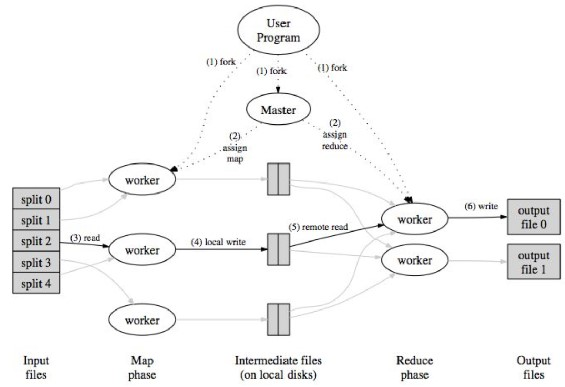
\includegraphics[scale = 2.0]{img/map reduce arch.jpg}
        \label{mr arch}
        \caption{MapReduce architecture}
\end{figure}

\begin{enumerate}
    \item The \textit{user program} invokes the MapReduce;
    \item The \textit{master node} coordinates the work. In particular, it assigns the \textit{workers} the splitting to which performing the Map function, and to other \textit{workers} the splitting to which performing the Reduce function and what intermediate files to read. The assignment of the chunks is usually based on the machine in which the chunk itself resides;
    \item The \textit{Map workers} read the split of the input files and they execute the Map function, writing the (key,value) output pairs into intermediate files in the local File System;
    \item The \textit{Reduce workers} read the intermediate files from the FS and execute the Reduce function, writing the final result into output files, which in turn can represent the input of another Map function.
\end{enumerate}

\subsubsection{Coordination and failures}
The coordination between all the workers is ensured by the \textbf{master node}. This data structure maintains the \textit{status} for each of the tasks (idle, in-progress, completed), and idle tasks get scheduled as workers become available. Moreover, when a Map task completes, it sends the master the location and size of its $R$ intermediate files, one for each reducer, and the master pushes these info to the reducers. Finally, another task of the master is to periodically ping the workers to detect failures.

A \textbf{failure} may happen on Map workers, on Reduce workers and on the Master node:

\begin{itemize}
    \item If a \textbf{Map worker failure} happens, then the Map tasks that are completed or in-progress are reset to idle, and the Reduce workers are notified when the task is rescheduled on another worker, in order to delete his local copy of the failed Map's data;
    \item If a \textbf{Reduce worker failure} happens, then only the in-progress tasks are reset to idle, since the results of the completed tasks are already saved in the distributed FS;
    \item If the \textbf{Master node} fails, then the MapReduce task is aborted, and the client is notified.
\end{itemize}

\subsubsection{Number of Map and Reduce jobs}
In general, we number $M$ of map tasks and $R$ of Reduce tasks are parameters to be tuned. A rule of thumb suggests that $M$ and $R$ should be larger than the number of nodes in the cluster, otherwise we would not exploit the parallelization. In general:

\begin{itemize}
    \item $M$ is determined by the number of input splits;
    \item $R$ is determined by the number of distinct key-value pairs, so on the data;
    \item Having several mappers and reducers may improve load balancing and it speeds the recovery from work failure, but on the other hand it increases the overhead given by the coordination between the different workers;
    \item Usually $R < M$, because the system has a maximum capacity of parallel reducers, so the reducers are executed in waves. The shuffling of the first wave is done in parallel with mappers, i.e. very early in the computation, but the shuffling of other waves is done later, so there's less communication/computation overlap.
\end{itemize}

\subsubsection{Some improvements}
Some improvements over the classic architecture of Picture \ref{mr arch} can be done:

\begin{itemize}
    \item We know that Map tasks on the same node will produce many pairs with the same key (an example is provided in Picture \ref{wc scheme}, where we have a node containing two pairs \textit{(Car, 1)}), so the idea is to save some network time by pre-aggregating the pairs at Map level by using the \textbf{combiners}. In this sense:

    $$
    \text{combine}(k_2, \text{list}(v_2)) = \text{list}(k_3, v_3)
    $$

    In the example, the result of the use of the \textit{combine} function is to have a pair \textit{(Car, 2)} before the shuffling phase. Notice that the \textit{combine} functionality usually exploits the Reduce function, if the Reduce function is commutative and associative.

    \item We know that the input of the Map tasks are created by contiguous splits of the input file, and for the Reducer we need to ensure that intermediate \textit{(k,v)} pairs with the same key end up at the same reducer. In this sense, the system uses a default \textbf{partition function}, e.g. $\text{hash}(key) \text{mod} R$, in order to ensure both a faster computation of the Reduce functions and load balance among the reducers. Notice that the partition functions may be overridden and customized.

    \item In order to shorten the total execution time and to ensure fault tolerant property of the system, the system enables the \textbf{back-up tasks}, i.e. tasks that are executed twice, in two different machines, and the result of the faster one is kept. This solution dramatically shortens the job completion time.
    
\end{itemize}

In general, it is useful to underline that the MapReduce framework is \textbf{not} adopted for \textbf{performances}, since for example the writes of the mapper to the disk produce a huge overhead, and in general the shuffle step represents the bottleneck of the system. The \textbf{advantage} of this framework is that the user is asked only to override two functions (sometimes, other functions are needed to be implemented, such as combiners, partitioners, etc..), but on the other hand \textbf{not everything can be implemented in terms of MapReduce}. For example, the \textit{all pairs similarity problem} requires to scan $N^2$ candidates, where $N$ is the number of documents in the collection, and experiments showed that for 60MB worth of documents, the framework would generate 40GB of intermediate data to be shuffled. Graph mining problems such as community detection and PageRank computation are hard problem for MapReduce too.

\subsubsection{Implementations of MapReduce}
There exist many methods for implementing a MapReduce framework:

\begin{itemize}
    \item \textbf{Hadoop}, which is an Apache project providing a Java implementation of MapReduce and relying on the HDFS (Hadoop Distributed File System), which is efficient and reliable. Hadoop only needs to copy Java libraries into each machine of the cluster;
    \item \textbf{Dryad & DryadLINQ};
    \item \textbf{Pig}, which provides a rich scripting language, which is then transformed into a chain of MapReduce jobs;
    \item \textbf{Hive}, which is a open-source data warehousing solution built on top of Hadoop, supporting queries in a SQL-like declarative language;
    \item \textbf{Spark}, which is a fast and general-purpose cluster computing system, that provides a high-level APIs in Scala, Java and Python, that make parallel jobs easy to write. It resolves around the concept of a Resilient Distributed Dataset (RDD), which is a fault-tolerant collection of elements that can be operated on in parallel
\end{itemize}

\subsection{Documents all pairs similarity with MapReduce}
The problem is defined as follows: given a collection of documents and a minimum required similarity threshold, the goal is to retrieve from the collection the number of pairs of documents that have a similarity greater or equal to the threshold value. In this case, each document is represented as a vector $d$ of $N$ elements, where $N$ is the size of the lexicon, and each $d[i]$ stores the \textit{tf-idf} value of term $i$ in the corpus. Moreover, the similarity is computed using the cosine similarity:

$$
s(a,b) = \sum_{i = 1, .., N} a[i] \cdot b[i]
$$

We now discuss a method for solving this problem exploiting the MapReduce framework. 

\subsubsection{First solution}
First of all, we can observe that the minimum requirement for two documents to have a similarity greater than 0 is to have at least one term in common, so the idea is to skip the computation of the similarity for two documents that do not have any term in common. In this sense, if we store, for each term in the lexicon, the list of documents containing that term, we can easily compute the similarity between these documents.

$$
(\text{term}_1, [\text{doc}_1, \text{doc}_2, ..])
$$

Thus, the \textbf{Reduce function} works like this: it receives in input a key-value pair, where:

\begin{itemize}
    \item the key is represented by the term;
    \item the value is represented by the list of documents in which the term appears.
\end{itemize}

, and for each pair of documents in which each term in the lexicon appears, it computes the similarity and it compares it with the threshold value. Thus, it never computes the cosine similarity of documents that do not contain any term in common. 

Once we designed the Reduce function, we must design the Map and the Shuffle functions. The \textbf{Map function} produces, for each term in the lexicon, a key-value pair where:

\begin{itemize}
    \item the key is represented by the term;
    \item the value is represented by a tuple (docID,document), where document represents the full document;
\end{itemize}

Then, the \textbf{Shuffle function} simply performs a GroupBy operations by key, i.e. by term, and it produces the key-value pairs that are given in input to the Reduce function. Picture \ref{mr all pairs} shows the Map and the Reduce functions for this problem.

\begin{figure}[h!]
		\centering
		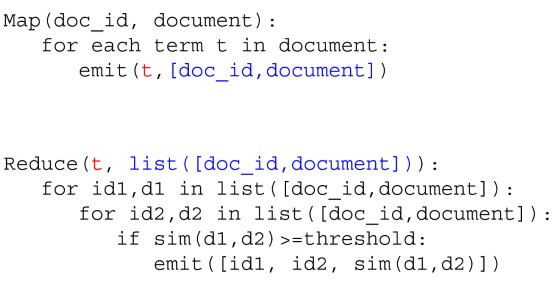
\includegraphics[scale = 2.0]{img/map reduce all pairs.jpg}
        \label{mr all pairs}
        \caption{Map and Reduce functions for all pairs similarity}
\end{figure}

Picture \ref{mr ex} shows an example of the functioning of the MapReduce framework for this problem.

\begin{figure}[h!]
		\centering
		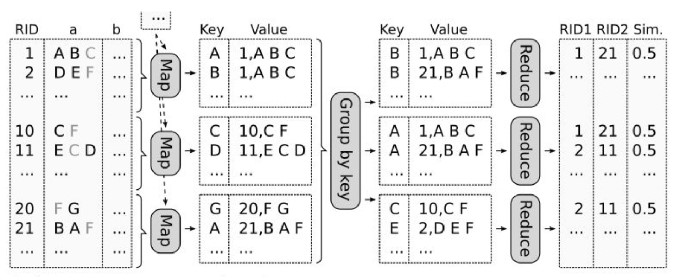
\includegraphics[scale = 2.0]{img/mr ex.jpg}
        \label{mr ex}
        \caption{Example of MapReduce functioning for all pairs similarity}
\end{figure}

However, a \textbf{first problem} is the following one: if a document has 1,000 terms, then the document is replicated 1,000 times after the Map execution.

\subsubsection{Second solution}
In order to solve the previous problem, we implement the so called \textbf{prefix filtering}. The idea is to reduce the number of terms we consider, in order to reduce the number of pair for which the similarity is computed.

\begin{enumerate}
    \item First of all, if we consider the term-document matrix, we sort the terms by decreasing score in the corpus, i.e. $d[0]$ corresponds to the term having the largest score of \textit{tf-idf};
    \item Then, we create the \textit{maximum document} d*, i.e. $d^*[i] = \max d[i]$ for each $d$ in the collection. In other words, $d^*$ stores the maximum score of terms in any document. Now we can have \textbf{two observations}:

    \begin{itemize}
        \item If $\text{sim}(d,d^*) < \text{threshold}$, then $d$ has no similar documents in the corpus. This is true because $d^*$ represents the maximum document, so for sure it does not exist another document $d_j$ s.t. $\text{sim}(d, d_j) \geq \text{threshold}$;
        \item Suppose we arrive at a certain term, and $\text{sim}(d,d^*) < \text{threshold}$: then, we can find another document $d_j$ similar to $d_i$ only if they have a term in common after the term we're now considering, otherwise we now that it does not exist another document $d_j$ s.t. $\text{sim}(d, d_j) \geq \text{threshold}$ form the above observation. In this sense, all the terms up to the current one are useless, so we only consider the other in the Map function. In other words, the Map function only considers the terms $t > b(d)$, where $b(d)$ is the \textit{boundary} of a document s.t.:

        $$
        \sum_{0 \leq t \leq b(t)} d[t] \cdot d^*[t] < \text{threshold}
        $$

        , i.e. the boundary of each document is represented by the largest term for which we have $\text{sim}(doc, d^*) < \text{threshold}$
    \end{itemize}
    
\end{enumerate}

Picture \ref{mr all pairs2} shows the Map and Reduce functions for this version of the solution.

\begin{figure}[h!]
		\centering
		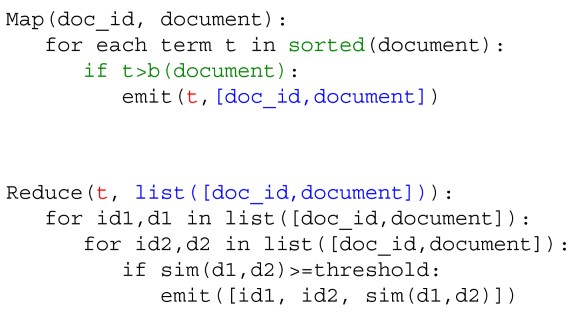
\includegraphics[scale = 2.0]{img/mr ex2.jpg}
        \label{mr all pairs2}
        \caption{Map and Reduce functions for all pairs similarity with prefix filtering}
\end{figure}

However, we have another \textbf{problem}: if two documents share 10 terms after filtering, then their similarity is computed and produced in output 10 times.

\subsubsection{Third solution}
A possible solution for this new problem could be sort the whole output and remove the duplicates, but we can easily notice that it is quite expensive.

For this reason, another approach is based on the following idea: only one Reducer is forced to compute the similarity. However, if the two documents are replicated 10 times with 10 different keys, they may end up in 10 different Reducers, so how do we tell the Reducers whether to compute or not the similarity? A selection mechanism can be exploited, e.g. if the reducer has the key equivalent to the largest item, it can compute the similarity.

\begin{figure}[h!]
		\centering
		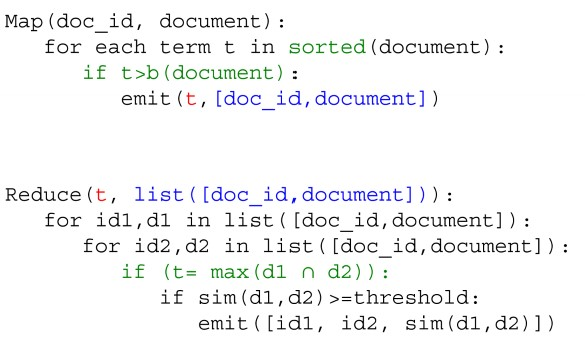
\includegraphics[scale = 2.0]{img/mr ex3.jpg}
        \label{mr all pairs3}
        \caption{Map and Reduce functions for all pairs similarity with improved prefix filtering}
\end{figure}

Picture \ref{mr all pairs3} shows the Map and Reduce functions for this version of the solution.

\subsection{Graph mining problem with MapReduce}
We consider an undirected graph, and our goal is to find the \textbf{number of connected components}, possibly exploiting the MapReduce framework. In general, graph mining problems are difficult to be parallelized, because, for example, if we think of the "divide-et-impera" approach, we have to partition the graph (i.e. breaking connected components), run the algorithm on each sub-graph and merge the partial results. In this sense, we now exploit a different paradigm of computation, the \textbf{vertex centric paradigm}.

The idea of this paradigm is to write an algorithm for a node rather than a graph, i.e. we specify what each node has to do. In particular, the sketch of the algorithm is the following:

\begin{itemize}
    \item Each node knows about its neighbors and may hold some additional custom information;
    \item The same computational kernel is executed for each node;
    \item Repeat until convergence.
\end{itemize}

The \textbf{advantages} of of this paradigm are:

\begin{itemize}
    \item It is easier to design a "local" algorithm for a single node, rather than for the entire graph;
    \item We can exploit a large parallelism degree, since each node is independent from the others;
    \item It can be implemented over MapReduce, and there exist some specific frameworks like Spark GraphX.
\end{itemize}

However, a \textbf{disadvantage} is that the local view may lead to sub-optimal results.

\subsubsection{Label propagation}
We now describe the algorithm we introduced in the previous section. 

The \textbf{input} of the algorithm is a list of $(X,C_{\text{min}})$ pairs, meaning that $X$ belongs to the connected component with id $C_{\text{min}}$: clearly, when the algorithm starts, node $X$ belongs to component with id $X$. Moreover, each node knows its neighbors $N(X)$.

The algorithm works as follows:

\begin{enumerate}
    \item Node $X$ sends its own component id $C_{\text{min}}$ to all its neighbors $N(X)$, along with itself. In this sense, each node outputs a $(X, C_{\text{min}})$ pair;
    \item Node $X$ receives a list of component ids and computes the minimum among them, i.e. the new $C_{\text{min}}$;
    \item Repeat until convergence, i.e. when no updates occur.
\end{enumerate}

As we said before, the idea of the algorithm is at each step, each node shares its own information to the neighbors, and the information shared by a node may eventually reach all the nodes of the connected component.

Picture \ref{lab prop} shows an example of the execution of Label Propagation.

\begin{figure}[h!]
		\centering
		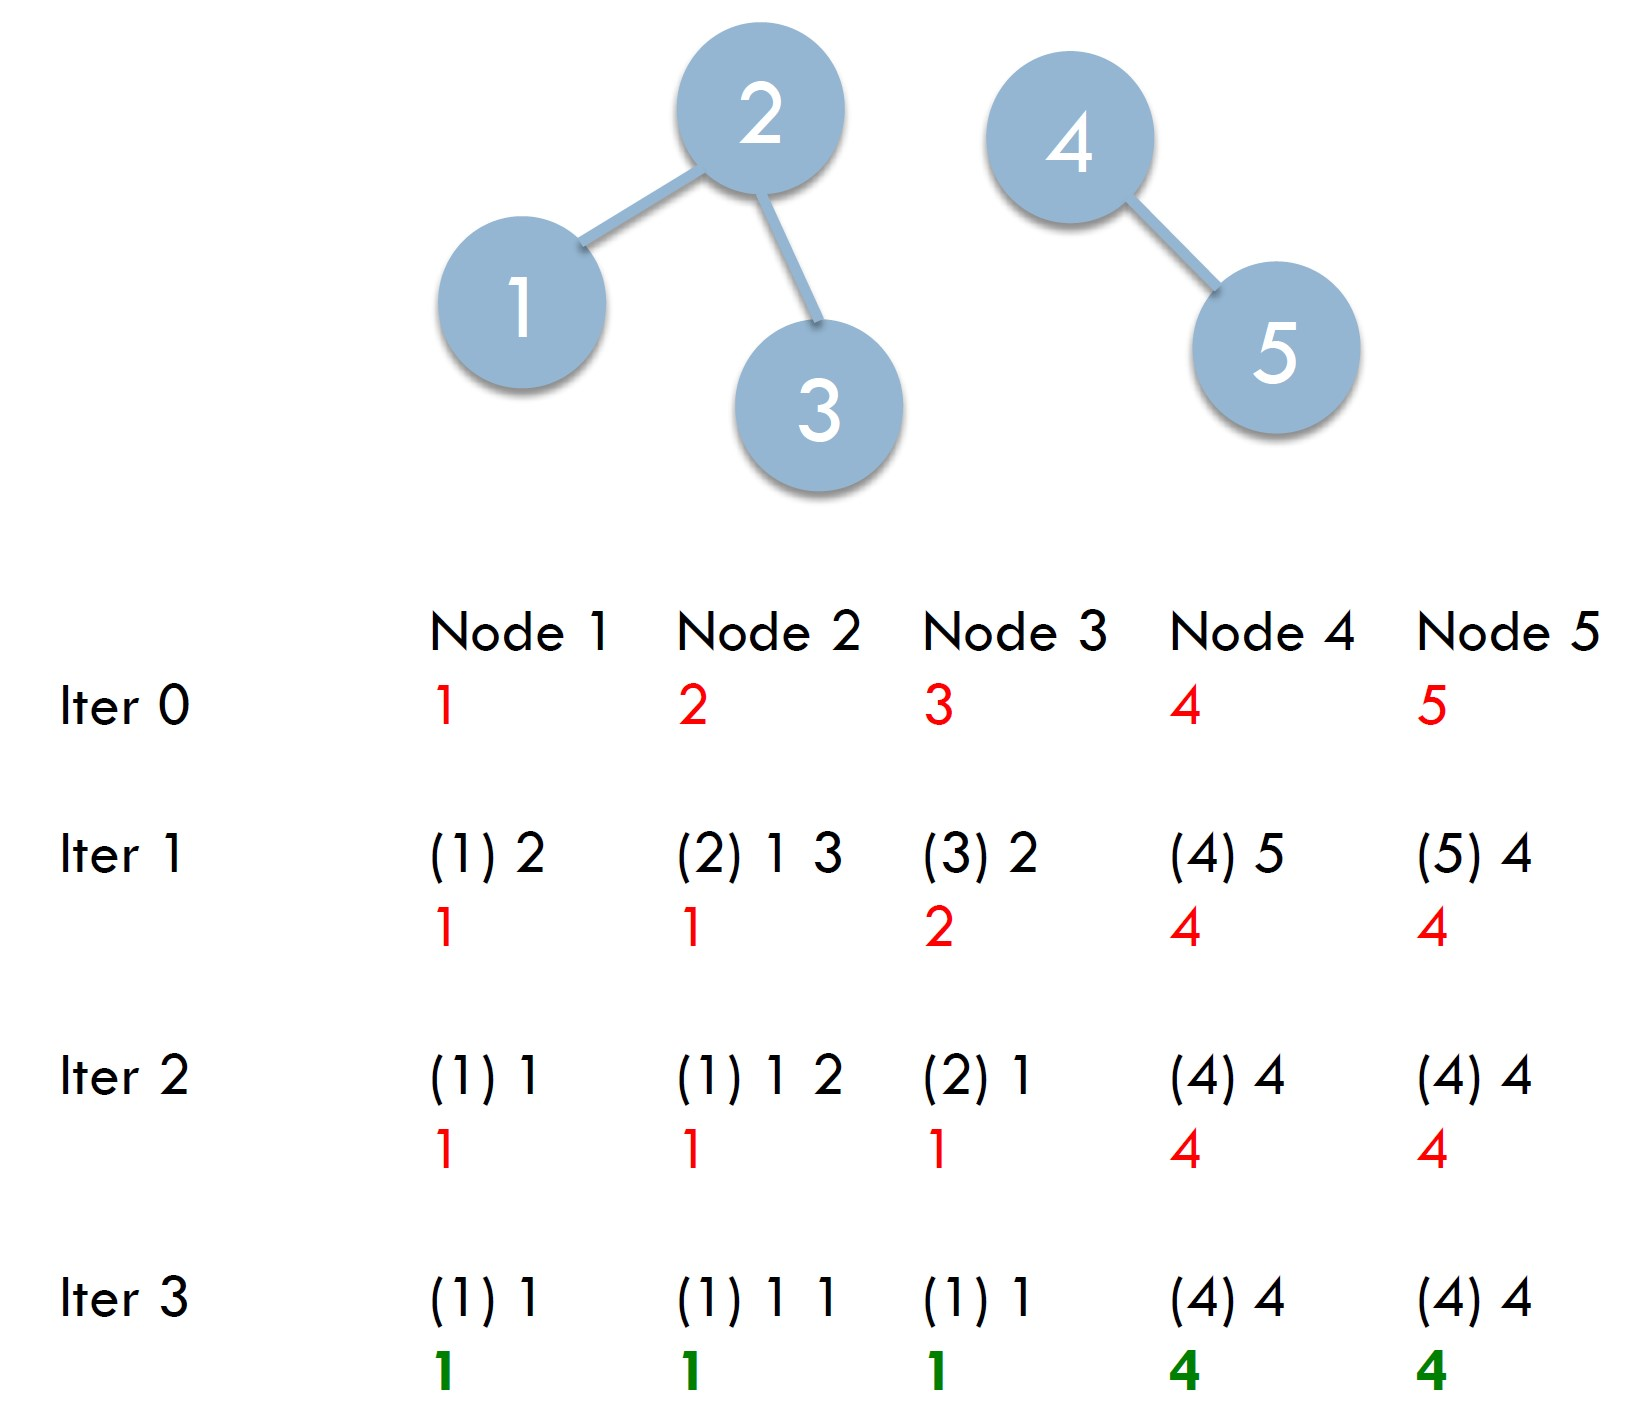
\includegraphics[scale = 0.5]{img/label propagation.jpg}
        \label{lab prop}
        \caption{Example of Label Propagation execution}
\end{figure}

As we can see, the initial value of $C_{\text{min}}$ is $X$ itself. In the first iteration, node 1 receives the component id of node 2, while node 2 receives the component ids of both node 1 and 3, and so on. Now, the minimum of such received component ids in computed, and the spread operation is repeated until convergence. In the end, the two connected components are retrieved.

Notice that this algorithm well adapt the MapReduce framework, since:

\begin{itemize}
    \item The Map function produces a list of $(\text{destination}, \text{message})$ pairs, where the \textit{destination} is the destination node of the \textit{message} that is spread at each iteration;
    \item The Shuffle function simply performs a GroupBy operation by key, in this case by \textit{destination}, so all the messages for each destination node are collected;
    \item The Reduce function produces a list of $(\text{destination}, \text{minimum value})$.
\end{itemize}

Notice that the \textbf{complexity} of the algorithm depends on the size of the largest connected component(s).

\subsubsection{Hash-To-Min}
We now discuss another algorithm for collecting the connected components of a directed graph.

In this case the \textbf{input} of the algorithm is given by a list of $(X,C)$ pairs, meaning that $X$ knows about nodes in the set $C$: clearly, when the algorithm starts, the set $C$ is composed of the node $X$ and its neighbors.

The algorithm works as follows:

\begin{enumerate}
    \item Node $X$ computes $C_{\text{min}}$, the smallest node in $C$;
    \item Node $X$ sends $C$ to node $C_{\text{min}}$;
    \item Node $X$ sends $C_{\text{min}}$ to any other node in $C$;
    \item Node $X$ creates a new $C$ by merging all the received messages;
    \item Repeat until convergence.
\end{enumerate}

Picture \ref{htm} shows an example of the execution of Hash-To-Min. As we can see:

\begin{itemize}
    \item When the algorithm starts, each node knows about itself and its neighbors;
    \item At iteration 1, each node computes $C_{\text{min}}$, and sends $C$ to $C_{\text{min}}$: node 1 sends (1,2) to itself, while it receives (1,2,3) from node 2. Then, each node sends $C_{\text{min}}$ to any other node in $C$: node 1 sends 1 to node 2, while node 2 sends 1 to node 3 etc..;
    \item At the end of each iteration, each node merges the received messages, and the operation are repeated until convergence.
\end{itemize}

Note that in this case the complexity is $O(\log d)$, where $d$ is the diameter of the graph: the idea is that at each iteration the information of each node nearly doubles.

\begin{figure}[h!]
		\centering
		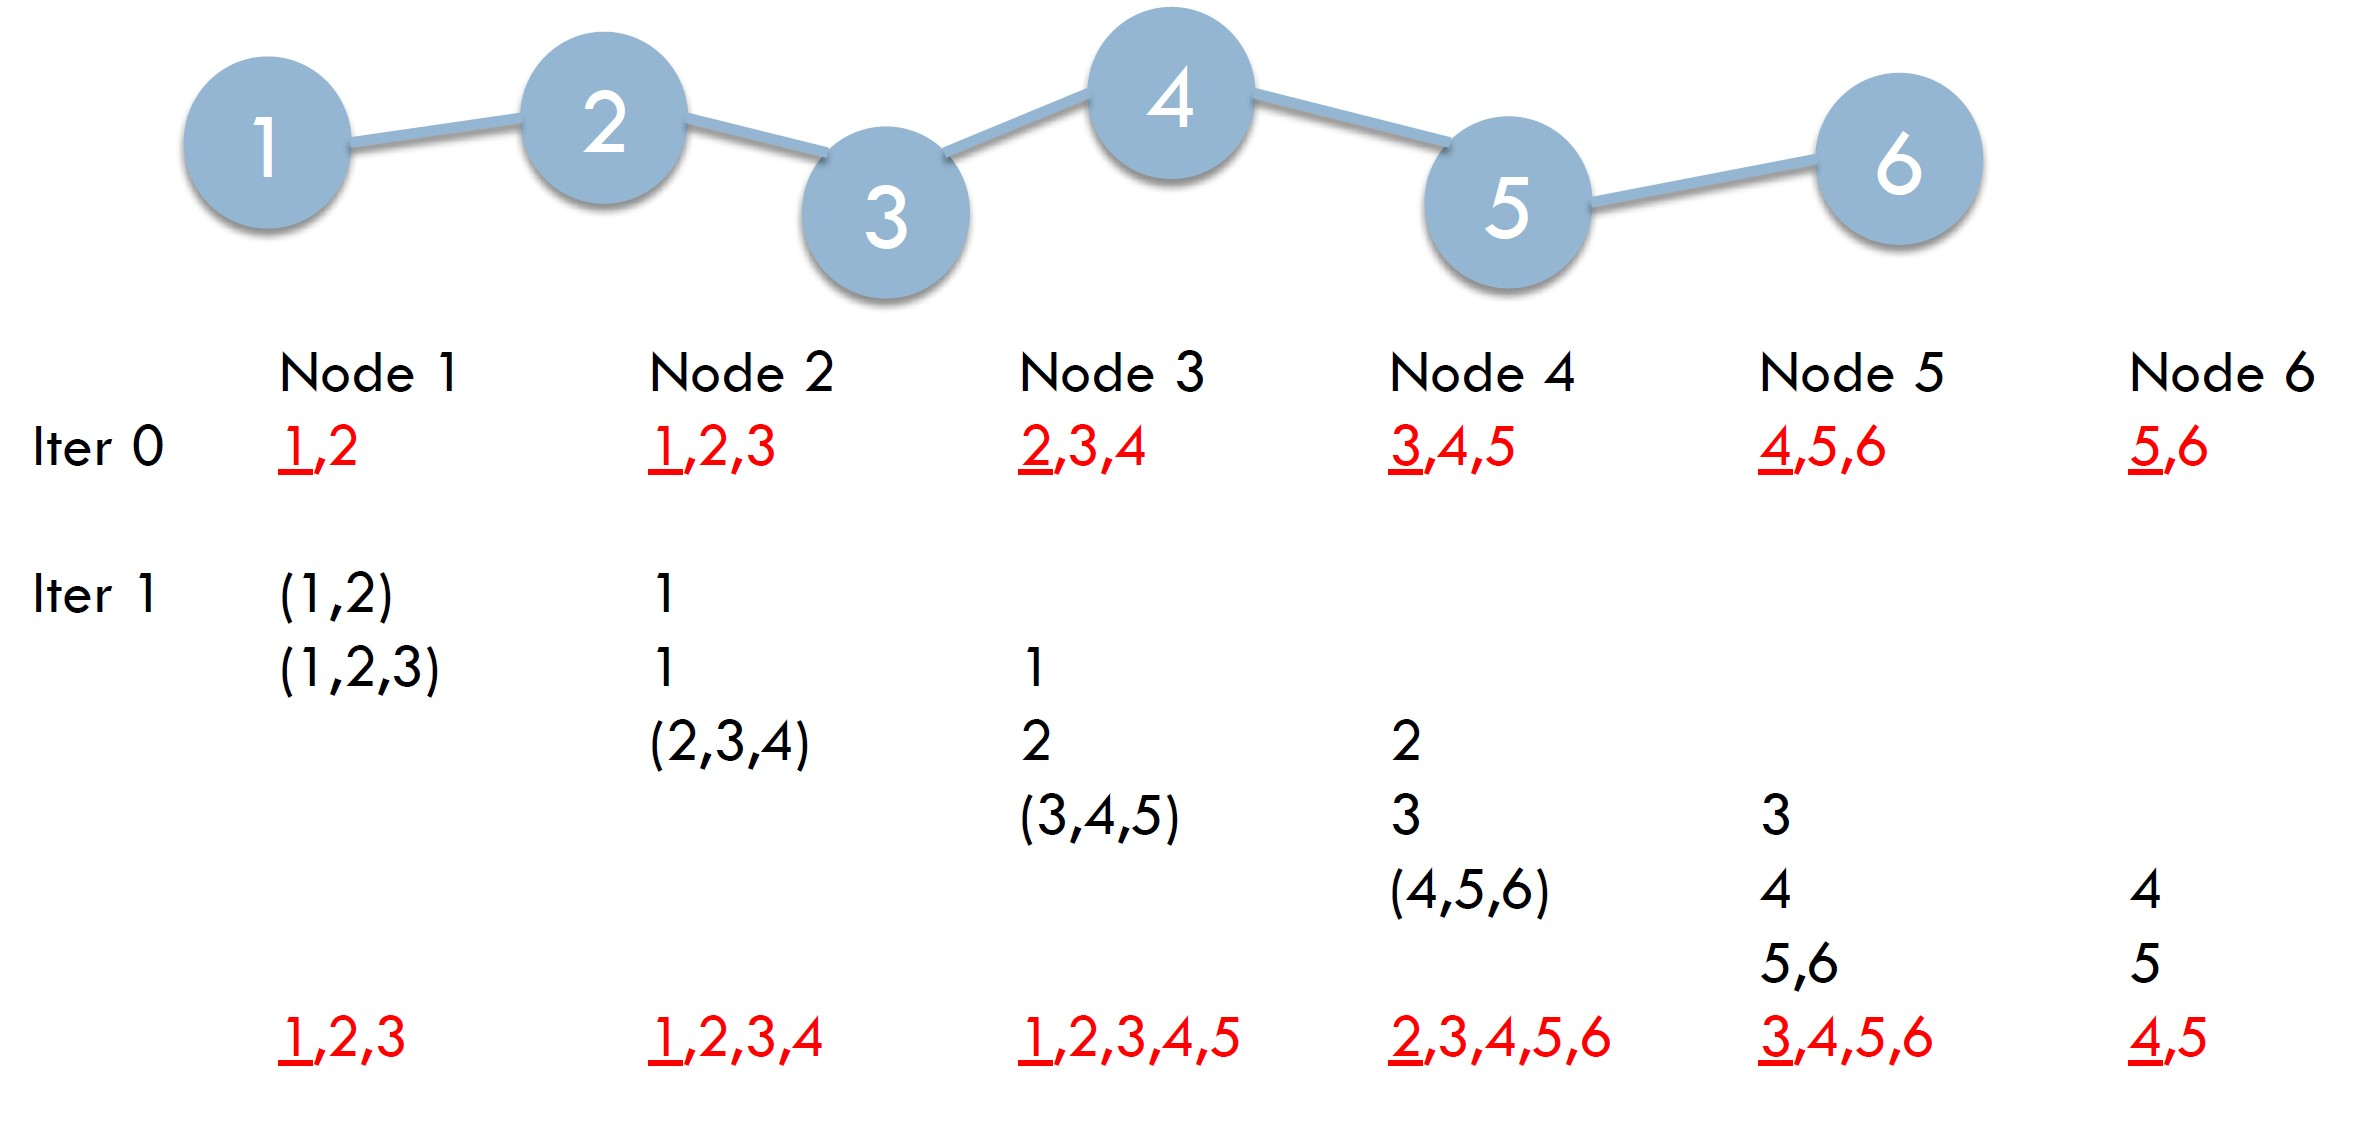
\includegraphics[scale = 0.5]{img/htm1.jpg}
        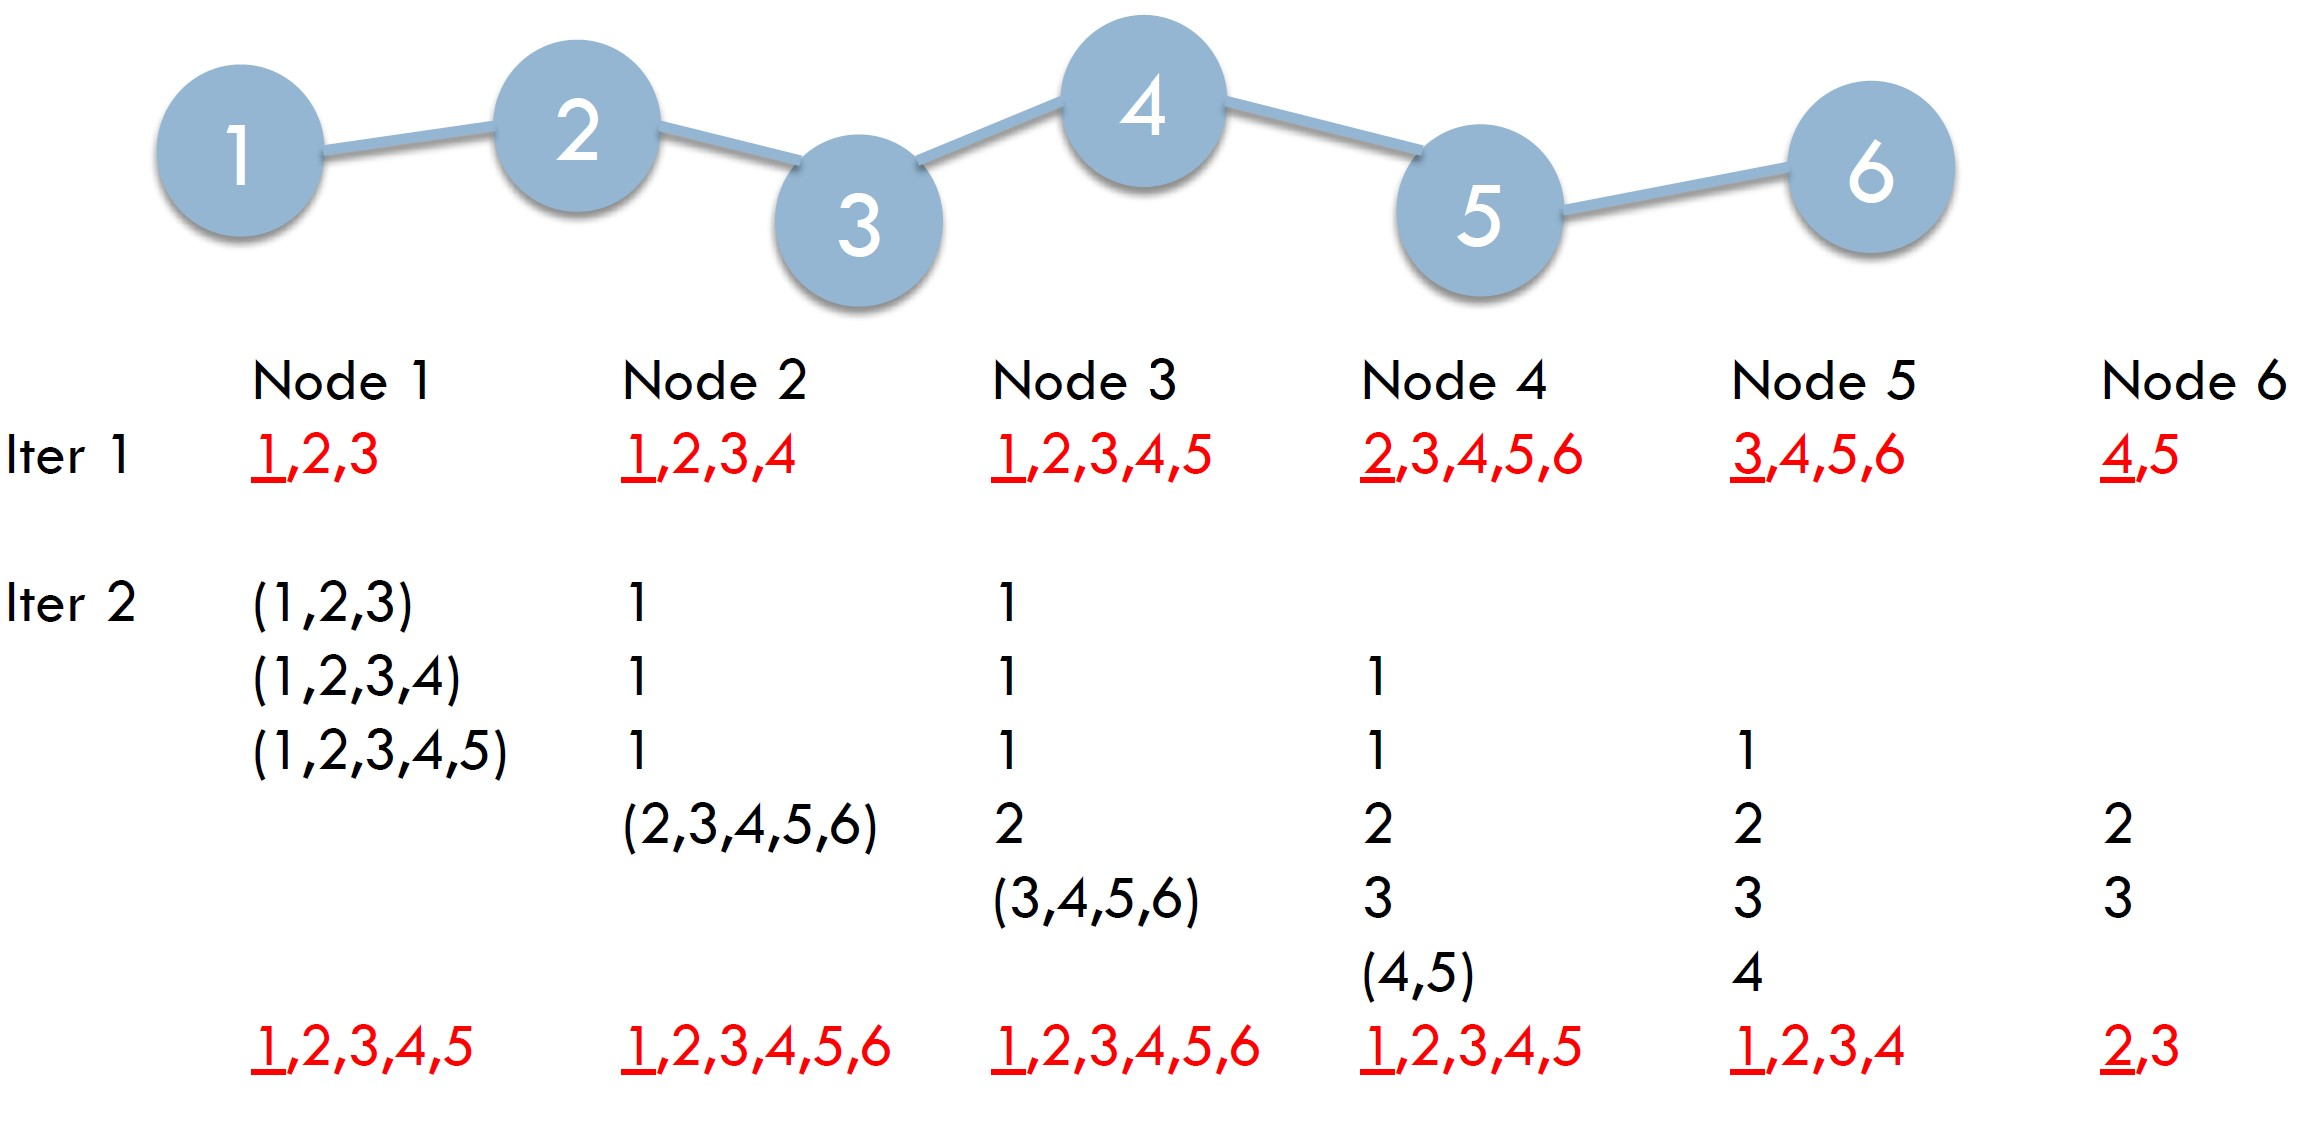
\includegraphics[scale = 0.5]{img/htm2.jpg}
        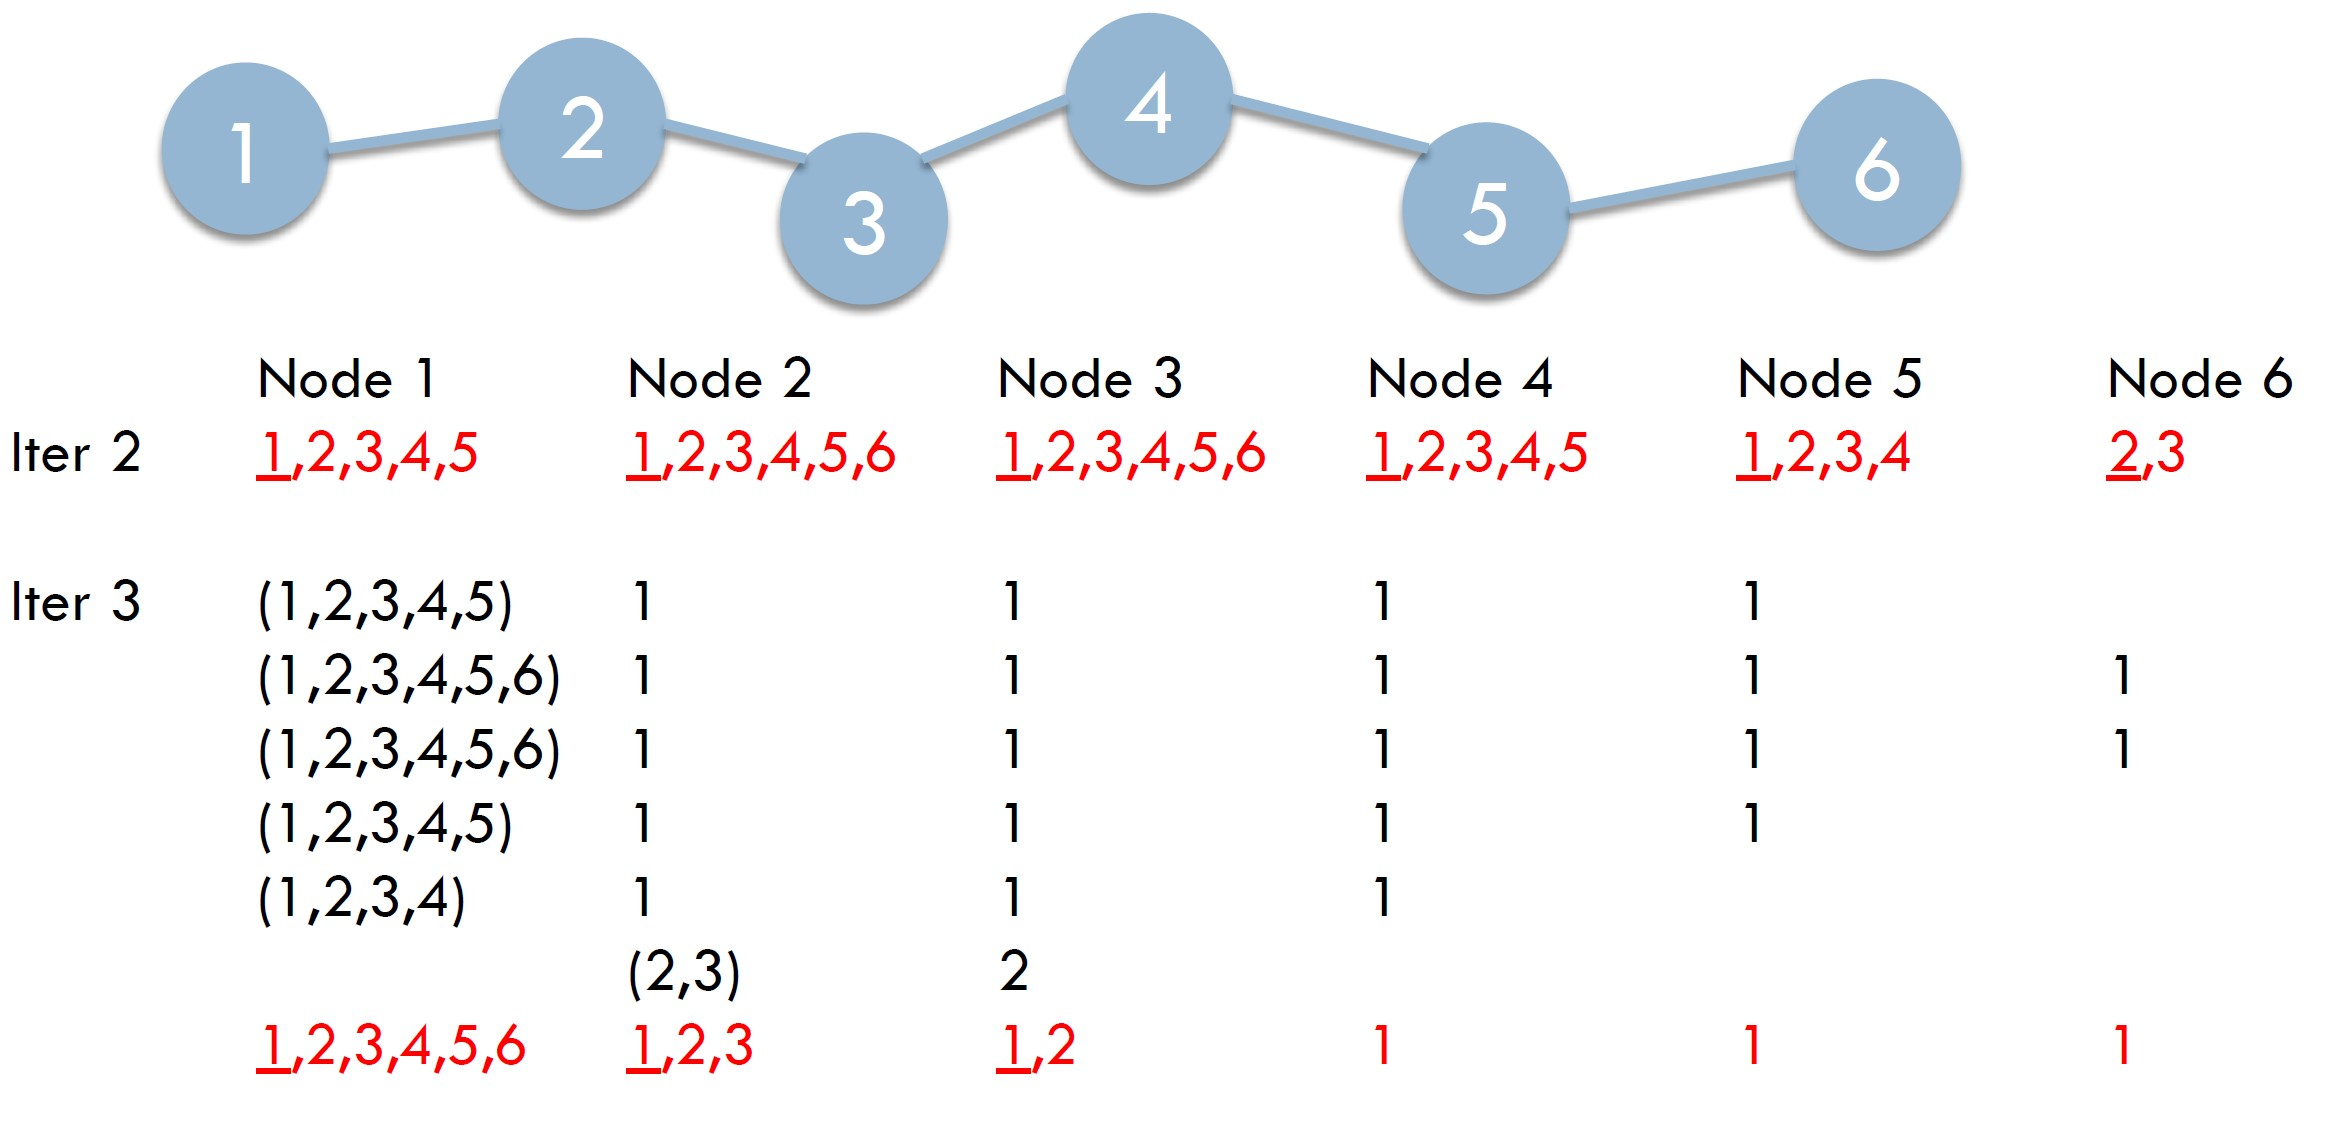
\includegraphics[scale = 0.5]{img/htm3.jpg}
        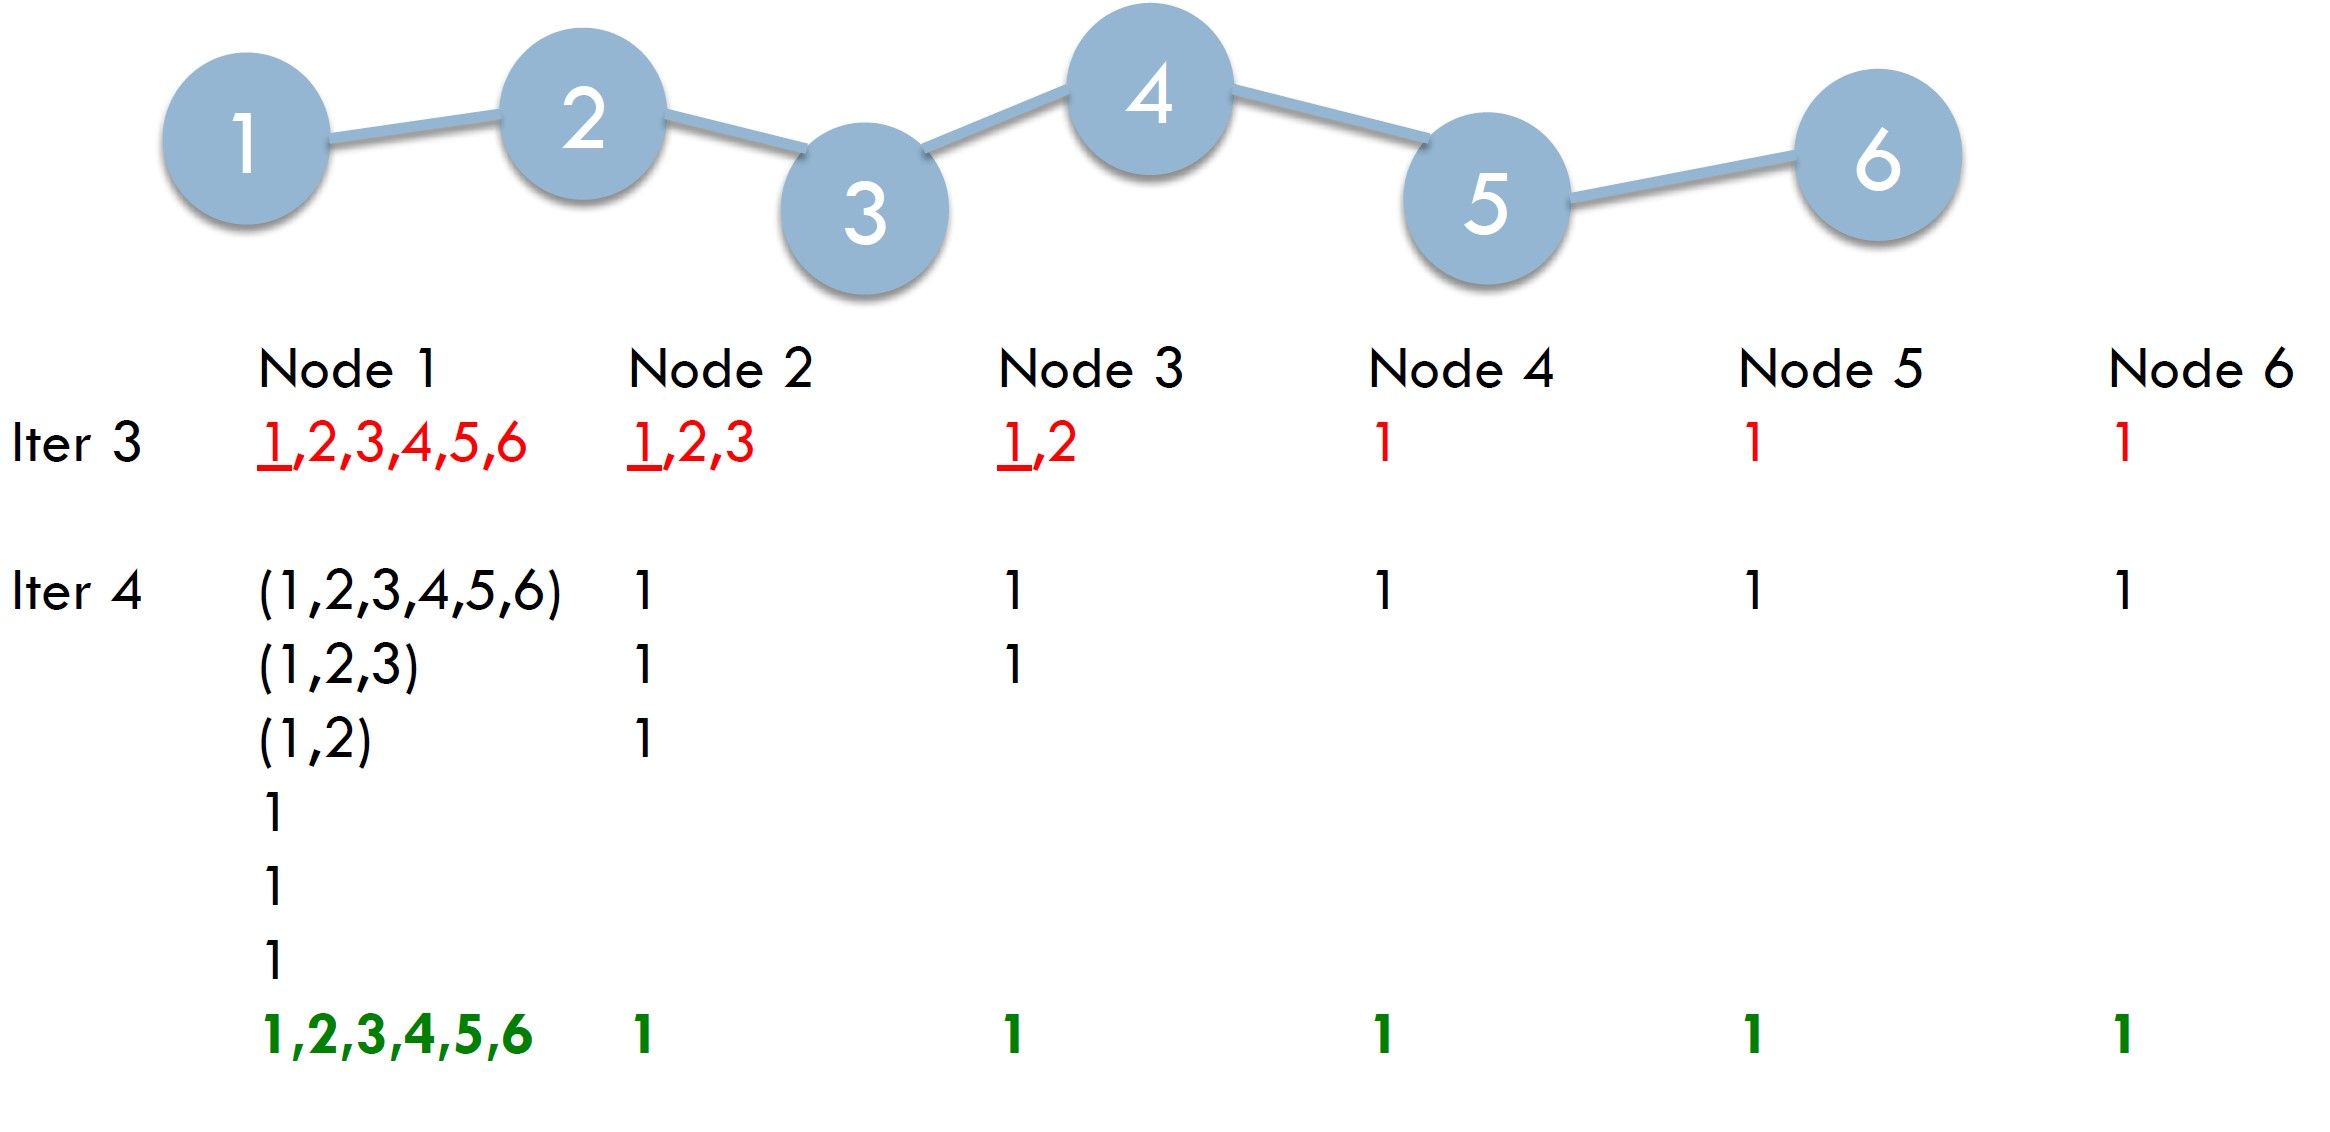
\includegraphics[scale = 0.5]{img/htm4.jpg}
        \label{htm}
        \caption{Example of Hash-To-Min execution}
\end{figure}